% This section includes some motivations behind the work, explicitly or implicitly highlights the research question , provides a high-level explanation of the solution, and describes the contributions.

% establish the context, background and/or importance of the topic
In the current global economy, the financial fraud has become a crucial issue especially for the trade sector. In recent times, the number of fraud cases have increased drastically which effected both financial institutions and their clients significantly. From a survey in 2020 on economic crime and fraud by Price Waterhouse Coopers, its been reported that more than 42 billion USD of financial losses happened in past 24 months~\cite{PwC.Crime.Survey}. On an average companies reportedly experienced 6 fraud cases during this period. Thirty five percent of fraud cases are marked as Customer fraud~\cite{PwC.Crime.Survey}.   

In current trend, more and more, companies outsource non-core activities to third party companies to reduce operational costs. But these third party-party business partners can be fraught with risk. One in five respondents from the PwC survey~\cite{PwC.Crime.Survey} cited vendors/suppliers as the source of their most disruptive external fraud. On the other hand, suppliers are also in high risk of fraud cases from their buyers. Due to this detecting suspicious companies (buyers and suppliers) plays an important role to reduce financial losses for the trade insurance companies and theirs customers.



% brief synopsis of the relevant literature
Fraud or extortion is a par of internal threats for any business. Manufacturers and service providers may face financial losses from fraudulent buyers. According to Association of Certified Fraud Examiners ACFE, the definition of fraud is \"the use of one’s occupation for personal enrichment through the misuse or deliberate
misapplication of the resources or assets of the employing organization~\cite{kassem_2014}. To term fraud that is imposes to manufactures and service provider it can be redefined as the personal gain of the buyers by misuse or deliberate misapplication of the products and services of the supplying organization and their respective insurance companies.

\begin{figure}[htp]
    \centering
    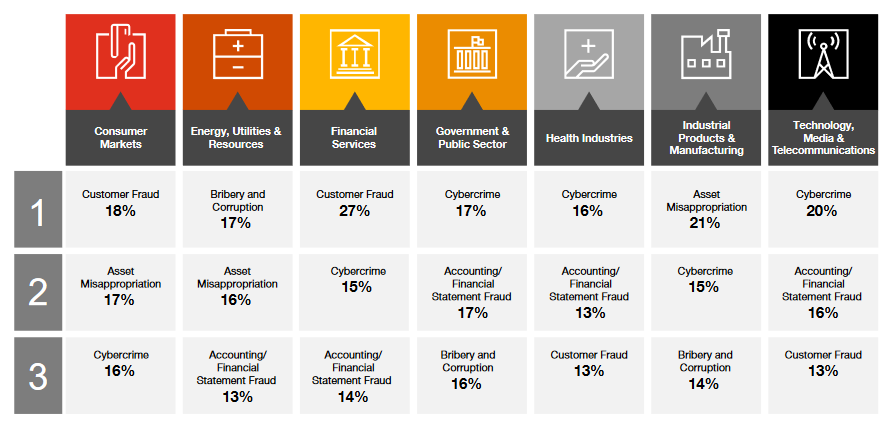
\includegraphics[width=\linewidth]{figures/fraud_by_industry.PNG}
    \caption{Most disruptive fraud events – by industry.Source: PwC 2020 Fraud survery~\cite{PwC.Crime.Survey} }
    \label{fig:fraud_sector}
\end{figure}
% Indicate an issue, problem or controversy in the field of study

A classical approach to prevent such fraudulent cases is done by traditional method of using human resources like internal and external auditors~\cite{kassem_2014}, and business team. Each team has their own process of monitoring external partners and buyers by analyzing transaction patterns, financial overview, historical behaviour to identify suspicious companies.  Based on the organizational capabilities, these team uses different internal and external resources like archival system, reports and news source.


Historically, organizations and financial institutions are using different technological solutions and operational process to detect suspicious companies. In the technological solutions different software are used to verify names, previous history and financial status of the buyers. On the other hand, as part of operational process during the customer on-boarding the Know Your Customer KYC process are used to identify anomaly in the customer profile. However, the major problems for these existing solution to detect suspicious companies are complex, time consuming, costly,and cognitively challenging labour intensive task.


However, in recent past with the advancement of artificial intelligence and data mining techniques, different machine leaning solutions are developed to find anomalies, credit card fraud, etc.~\cite{RB2021, KIRKOS2007995}. Considering the complexity of the tasks the continuous improvement of the systems are going on. The incremental success of these solutions are showing a great promises to reduce operations time and cost for the organizations and financial institutions.

Most studies in the field of suspicious activity classification for economical sector are done on Credit Card fraud detection. The recent number of individual and organized criminals the number of credit card has increased significantly ~\cite{RB2021}. Although lots of research has been carried out on detecting anomalies in financial crime, we can see that most of the researches for identifying suspicious financial crime activity are focused on detecting credit card fraud. However, as mentioned earlier, in the survey from PwC we have seen that third party business crime and fraud imposes high risk and have huge financial impact on the economy.
% listing the reasarch question or hypotheses


This paper will focus on using a data-driven approach using machine learning techniques to detect suspicious companies to prevent financial losses for the organizations and respective financial institutions.  The major objective of this study is to use data mining technique to extract features from unstructured data, and apply ensemble learning and neural network to identify the pattern on the features to detect suspicious companies.

% provide synopsis of the research methols



Data extracted is a useful method to gather data for analysing and prediction tasks. Data driven is a method base on the history data to build more hyper-parameters to compensate the un-measurable features within the measurable data \cite{SMARRA20181252}. some extending nonlinear features to build the prediction function. In classification and prediction problem, it is essential to discover the pattern of the data and provide us some insights to take some actions according to the prediction results. Random Forest algorithm and Neural Networks are been used in handling this problem and shown effective~\cite{10.1145/3414274.3414278, RB2021}. However it is extremely hard to identify the target information from institutions data based on pattern. The propose of the paper is to find a suitable classifier and its application to find fraudulent cases based on assembly learning and machine learning .

\mytodo{update this text}



% Significance of value of the study


This thesis provided an important opportunity to advance the understanding of data-driven approach for extrapolate data from historical archive based on expert opinion. Also the paper covers how a real-world data with high class imbalanced is used for different machine learning approaches. The paper also tries to explain the complexity and challenges of identifying anomalies in the data set and share a practical overview on how to approach suspicious recommendation engine can be applied this financial and other suitable sectors.



% Define the topic or key term


Throughout this paper, the term Artificial Neural Networks, Random Forest, XGBoost, receiver operating characteristic, and are under the curve will refer to ANN, RF, XG, ROC and AUC. The term fraud is used interchangeably with suspicious activity done by companies to gain financial gain.

% Overview of teh report stucture


The main question address in this paper are:
\begin{itemize}
    \item[a.] Data driven approach to extract relevant information related to detecting suspicious behaviour or patters of companies
    \item[b.] Choosing the most appropriate model for detecting suspicious companies to prevent fraudulent cases.
\end{itemize}

To overall structure of the design takes the form of three steps. In step 1 a data driven technique is used to identify the most significant information based on the feedback from expert then extracting the information from historical dataset. In step 2 ensemble models and neural networks are used for suspicious companies classification problem. And last but not least, in step 3 Different machine learning metrics are used to select the best performing model. The details of the approach are described in the overview [section: ~\ref{sec: Overview}] and design [sec:~\ref{sec: Design}] section of this paper.
% State the purpose of the essay / write


The case study of identifying suspicious companies that presented in this paper is conducted for one of the leading trade insurance company. The interested company has foot print over different locations in the world. The target of the company to reduce risk by preparing a classification model which recommends or detects suspicious companies to prevent itself from having financial loss due to fraudulent activity.
% Provide an overview of the coverage


Designing and setting the suitable machine learning model is a repetitive process. In this paper only section method of first model is described. Due to practical constrain not all other machine learning models and configuration of assembly models and neural networks are discussed. Also due to protect the internal process of the expertise of the insurance company have been excluded while describing the feature. However in the design section a generalized approach and pseudo code have been shared in section:~\ref{sec: Design}]






